\section{PROJE'NİN İŞLEYİŞİ}
\subsection{Arayüz Kısmı }
\subsubsection{Template Hazırlığı:}
Proje için uygun bir template seçilmiş ve projenin gereksinimlerine uygun hale getirilmiştir. Template içerisinde yer alan gereksiz kısımlar temizlenerek sağ menü bölümü oluşturulmuştur. Bu sayede kullanıcılar, sağ menü üzerinden kolayca erişebilecekleri Dashboard, görevler (Ping, Theharvester), sistem logları ve Profil gibi önemli bölümlere ulaşabileceklerdir. Bu düzenlemeler, arayüzün daha kullanıcı dostu ve projeye özgü hale getirilmesini sağlamaktadır.
\subsubsection{Kullanıcı Girişi:}
Projeyi ilk açtığınızda, kullanıcı login sayfasıyla karşılaşacaksınız. Bu sayfada kimlik bilgilerinizi girdikten sonra doğrulama işlemi gerçekleştirilir ve başarılı bir şekilde doğrulandığınızda diğer sayfalara erişim sağlanır. Bu sayede projenin güvenliği ve kullanıcı gizliliği sağlanırken, yetkilendirme mekanizması sayesinde sadece yetkili kullanıcılar projenin içeriğine erişebilir. Bu işlem, kullanıcıların projenin sunduğu özelliklere erişebilmeleri ve projeyi kullanmaya başlayabilmeleri için önemli bir adımdır.
\subsubsection{Kontrol Paneli:}
Giriş yaptıktan sonra karşılaşacağınız ilk sayfa Kontrol Paneli olacaktır. Kontrol paneli, kullanıcılara projede gerçekleştirilebilecek işlemleri açıklayan ve sunan bir sayfadır. Bu sayede kullanıcılar, projenin farklı özelliklerini keşfedebilir, verileri yönetebilir, raporları görüntüleyebilir veya diğer kullanıcılarla etkileşimde bulunabilir. Kontrol paneli, projenin merkezi bir noktasıdır ve kullanıcılara projenin sunmuş olduğu işlevselliği keşfetme ve kullanma imkanı sağlar. Bu sayede kullanıcılar projenin potansiyelini tam olarak kullanabilir ve projenin amaçlarına yönelik işlemleri gerçekleştirebilirler.
\subsubsection{Görevler Bölümü:}
Sağ menüde bulunan Görevler bölümünden, kullanıcılar yeni görevler oluşturabilir ve önceden oluşturulmuş görevlere erişebilirler. Görevler bölümü, kullanıcılara farklı işlemleri gerçekleştirmek için bir arayüz sağlar. Örneğin, bir Ping görevi oluşturulduğunda, kullanıcılar konteynırların çıktılarına, kayıp yüzdesine, maksimum, minimum ve ortalama geri dönüş sürelerine erişebilirler. Bu bilgiler, görevin durumu ve performansı hakkında önemli bilgiler sunar. Kullanıcılar, görevlerin sonuçlarını inceleyebilir, performans analizleri yapabilir ve gerektiğinde görevleri düzenleyebilirler. Görevler bölümü, kullanıcıların projede yapılan işlemleri izleme ve yönetme sürecine katkı sağlar, verimliliği artırır ve kullanıcılara kontrol sağlar.
\subsubsection{Sistem Logları:}
Sağ menüde bulunan Sistem Logları bölümü, kullanıcılara log kayıtlarını görüntüleme imkanı sunar. Bu log kayıtları, kullanıcının hangi görevleri ne zaman çalıştırdığını, görevlerin tamamlanma sürelerini, başarı durumunu ve oturum açma/kapatma bilgilerini içerir. Sistem Logları bölümü, kullanıcılara gerçek zamanlı olarak yapılan işlemleri takip etme ve denetleme yeteneği sağlar. Bu sayede kullanıcılar, projenin geçmişinde gerçekleşen işlemleri izleyebilir, performans analizleri yapabilir ve gerektiğinde sorun giderme yapabilir. Sistem Logları bölümü, kullanıcılara projenin izlenebilirliğini artırırken, işlemlerin güvenliğini ve bütünlüğünü de sağlar.
\subsubsection{Hesabım Bölümü:}
Hesabım bölümü, kullanıcılara profil düzenlemelerini gerçekleştirme imkanı sunar. Bu bölümde kullanıcılar, profil bilgilerini güncelleyebilir, şifrelerini değiştirebilir, iletişim tercihlerini yönetebilir ve gizlilik ayarlarını düzenleyebilir. Profil düzenlemeleri sayesinde kullanıcılar, kendi hesaplarını kişiselleştirme ve özelleştirme imkanına sahip olurlar. Bu şekilde, kullanıcılar projedeki profil bilgilerini istedikleri şekilde yönetebilir ve hesaplarını kendi ihtiyaçlarına göre ayarlayabilirler. Hesabım bölümü, kullanıcılara projedeki kişisel bilgilerini güncelleme ve yönetme kolaylığı sağlar, böylece kullanıcılar projede daha iyi bir kullanıcı deneyimi yaşayabilirler.

%arayüz fotoğrafları eklenecek 
\subsection{Arka plan işleyişi}
Projenin alt yapısı, PHP framework'ü olan Laravel kullanılarak geliştirilmiştir. Projenin çalışması için bir docker-compose.yml dosyası kullanılarak Docker'da bir servis oluşturulmuştur. Bu servis, iki konteyner oluşturarak projenin çalışmasını sağlamaktadır. Docker yönetimi için Docker Engine API kullanılmıştır.

\subsubsection{Docker Engine API}

Docker, Docker Engine API olarak adlandırılan arka plan programı sayesinde etkileşim için bir API sağlamaktadır. Docker Engine API, birçok modern programlama dilinde yer alan HTTP kütüphanesi tarafından erişilen bir RESTful API'dir. Projedeki PHP SDK güncel olmadığı için, Docker API'yi kullanarak Laravel uygulaması ile haberleşme sağlayan DockerService adında bir servis yazılmıştır. Bu sayede konteyner oluşturma, çalıştırma, detaylarını görüntüleme gibi işlemler yapılabilmektedir.

\subsubsection{Laravel Özellikleri}

Bu projede, Laravel'in sağladığı özellikler kullanılarak geliştirme yapılmıştır. Bir IP'ye ping atma görevi oluşturma süreci şu şekildedir:

Kullanıcı, ping oluşturma görevi formunu doldurmalıdır. Formda, görev başlığı, görev açıklaması, atılacak IP adresi, oluşturulacak konteyner sayısı ve her bir konteynerda kaç adet ping atılacağı gibi fieldler bulunmaktadır.

Form doldurulduktan sonra, PingRequest sınıfı devreye girecektir. Bu, Laravel'in sağladığı bir özellik olan Request'tir ve formdan gelen bilgilerin doğruluğunu sağlamaktadır. Eğer bilgiler doğruysa, PingController'a geçilir. Eğer bilgiler doğrulanamazsa, form sayfasına geri yönlendirilir ve eksik olan fieldlerin altında bir hata mesajı yazılır.

PingController, yeni bir görev oluşturarak kullanıcıyı görev listesi sayfasına yönlendirir ve "oluşturuldu" mesajını yazdırır.

Yeni bir görev oluşturulduğunda, Laravel'in bir diğer özelliği olan "Event (Tetikleyici) \& Listener (Dinleyici)" devreye girer.

Event \& Listener: Bu proje, yeni bir görev oluşturulduğunda event tetiklenir ve Listener çalışmaya başlar. Listener aracılığıyla DockerService çalıştırılır. Kullanıcıyı Form sayfasında bekletmemek için Listener kuyruğa alınır ve DockerService işlemi tamamlandıktan sonra görev durumu güncellenir. Başarılıysa 1, başarısızsa 2 olarak bildirilir
%ibrahim bu kısımda özet yazacak detaylandırılacak
 \subsection {Veritabanı kısmı İçin }
 MySQL veritabanı kullanılarak bir proje için optimize edilmiş bir veritabanı şeması oluşturuldu. Bu şema, "users" (kullanıcılar), "ping" (ping kayıtları) ve "pingcontainers" (ping konteynerleri) adında üç tabloyu içermektedir. Bu düzenleme, veritabanının performansını artırmak ve veri bütünlüğünü sağlamak amacıyla yapılmıştır.\\
"users" tablosu, kullanıcıların temel bilgilerini içerir ve her kullanıcıya birincil anahtar (ID) ile benzersiz bir kimlik atar. Ayrıca kullanıcı adı, e-posta adresi ve diğer ilgili bilgiler gibi sütunlar da içerir.\\
"pingcontainers" tablosu, kullanıcıların oluşturabileceği ping konteynerlerini temsil eder. Her konteyner birincil anahtar ile tanımlanır ve kullanıcıya ait olacak şekilde kullanıcı kimliği (user ID) ile ilişkilendirilir. Bu tablo, kullanıcının birden fazla konteyner oluşturabilmesine olanak sağlar.\\
"ping" tablosu, gerçekleşen ping olaylarını kaydetmek için kullanılır. Her ping kaydı, birincil anahtar ile tanımlanır ve bir konteynere (container ID) ve kullanıcıya (user ID) bağlanır. Bu ilişki, her ping kaydının hangi kullanıcı ve konteyner tarafından oluşturulduğunu gösterir.\\
Bu veritabanı şeması, kullanıcıların birden fazla konteyner ve görev oluşturabilmesini sağlar. Ayrıca, her görevin bir kullanıcı tarafından oluşturulduğu ilişkisi sayesinde veri bütünlüğünü korur.\\
Bu düzenleme, veritabanının daha etkili bir şekilde veri saklamasını ve verilere hızlı erişim sağlamasını amaçlamaktadır. Ayrıca, veri bütünlüğünü korumak için gereken ilişkileri de sağlamaktadır.\\
 \begin{figure}[]
    \centering
    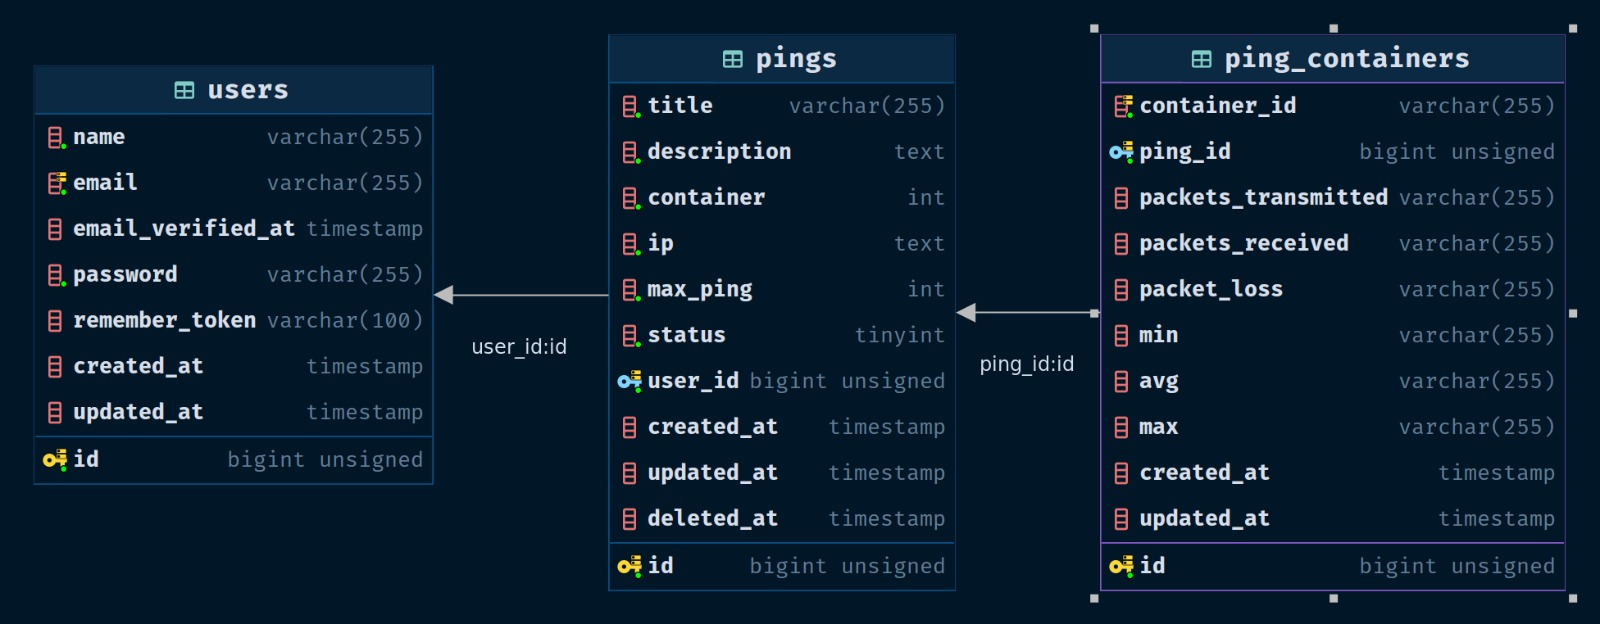
\includegraphics[width=0.9\textwidth]{images/sql.jpg}
    \caption{Sql ping tabloları}
    \label{fig:resim_etiketi}
  \end{figure}



